\documentclass{beamer}

\input{settings.tex}


\title{Algebra on three dimensions}
\subtitle{Math and modeling for high school, Lecture 3}
\author{by Sergei Savin}
\centering
\date{Fall 2022}



\begin{document}
\maketitle


%\begin{frame}{Content}
%
%\begin{itemize}
%\item Motivation
%\item Ordinary differential equations
%    \begin{itemize}
%    \item 1st order
%    \item n-th order
%    \end{itemize}
%\item Linear differential equations
%    \begin{itemize}
%    \item 1st order
%    \item n-th order
%    \end{itemize}
%\item Changing n-th order ODE to a State-Space form
%\item State-Space to ODE
%\item Read more
%\end{itemize}
%
%\end{frame}



\begin{frame}{Cross product}
	% \framesubtitle{Part 1}
	\begin{flushleft}
		
		Given two vectors $\mathbf a = [a_x \ a_y \ a_z]$ and $\mathbf b = [b_x \ b_y \ b_z]$, their cross product is:
		
		\begin{equation}
			\begin{bmatrix}
				a_x \\ a_y \\ a_z
			\end{bmatrix}
			\times
			\begin{bmatrix}
				b_x \\ b_y \\ b_z
			\end{bmatrix}
			=
			\begin{bmatrix}
				a_y b_z - a_z b_y \\ 
				a_z b_x - a_x b_z \\ 
				a_x b_y - a_y b_x
			\end{bmatrix}
		\end{equation}	
		
		Vector $\mathbf c = \mathbf a \times \mathbf b$ is orthogonal to both $\mathbf a$ and $\mathbf b$. Another definition of cross product is:
		
		\begin{equation}
			\mathbf a \times \mathbf b = ||\mathbf a|| \ ||\mathbf b|| \ \text{sin} (\varphi) \ \mathbf n 
		\end{equation} 
		
		where $\mathbf n $ is a unit vector, orthogonal to  both $\mathbf a$ and $\mathbf b$, whose direction can be determined with a right-hand-rule.
		
		
	\end{flushleft}
\end{frame}



\begin{frame}{Cross product}
	% \framesubtitle{Part 1}
	\begin{flushleft}
		
		Note two important properties of the cross product. First, if the angle between the two vectors is 0, meaning they are parallel, their cross product will have to be zero, since $\text{sin}(0) = 0$. This allows cross product to be used to detect linear dependence of two vectors in 3D.
		
		\bigskip
		
		Also, cross product can be used to produce a vector, orthogonal to a pair of other vectors.
		
	\end{flushleft}
\end{frame}



\begin{frame}{Planes}
	% \framesubtitle{Part 1}
	\begin{flushleft}
		
Consider a plane in 3D space, passing through the origin. We can characterize it with two vectors $\mathbf v_x$, $\mathbf v_y$ lying on it, and/or with a vector orthogonal to it $\mathbf v_z$. 

\bigskip

\tikzset{every picture/.style={line width=0.75pt}} %set default line width to 0.75pt        

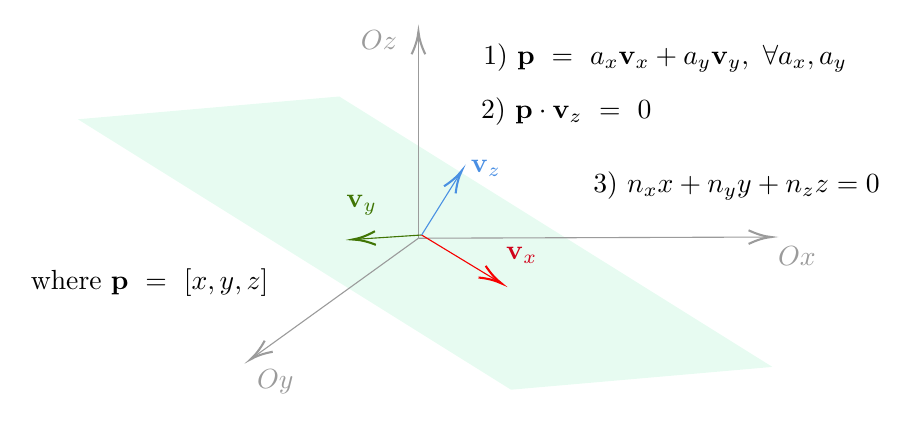
\begin{tikzpicture}[x=0.75pt,y=0.75pt,yscale=-1,xscale=1]
	%uncomment if require: \path (0,300); %set diagram left start at 0, and has height of 300
	
	%Shape: Parallelogram [id:dp236110485115546] 
	\draw  [draw opacity=0][fill={rgb, 255:red, 82; green, 230; blue, 155 }  ,fill opacity=0.14 ] (232.86,50.29) -- (441.53,180.58) -- (315.61,191.56) -- (106.94,61.27) -- cycle ;
	%Straight Lines [id:da6338056760294362] 
	\draw [color={rgb, 255:red, 155; green, 155; blue, 155 }  ,draw opacity=1 ]   (271,118.58) -- (439,118.01) ;
	\draw [shift={(441,118)}, rotate = 179.8] [color={rgb, 255:red, 155; green, 155; blue, 155 }  ,draw opacity=1 ][line width=0.75]    (10.93,-3.29) .. controls (6.95,-1.4) and (3.31,-0.3) .. (0,0) .. controls (3.31,0.3) and (6.95,1.4) .. (10.93,3.29)   ;
	%Straight Lines [id:da40408360827705025] 
	\draw [color={rgb, 255:red, 155; green, 155; blue, 155 }  ,draw opacity=1 ]   (271,118.58) -- (271,21) ;
	\draw [shift={(271,19)}, rotate = 90] [color={rgb, 255:red, 155; green, 155; blue, 155 }  ,draw opacity=1 ][line width=0.75]    (10.93,-3.29) .. controls (6.95,-1.4) and (3.31,-0.3) .. (0,0) .. controls (3.31,0.3) and (6.95,1.4) .. (10.93,3.29)   ;
	%Straight Lines [id:da5281297275813817] 
	\draw [color={rgb, 255:red, 155; green, 155; blue, 155 }  ,draw opacity=1 ]   (271,118.58) -- (191.62,175.83) ;
	\draw [shift={(190,177)}, rotate = 324.2] [color={rgb, 255:red, 155; green, 155; blue, 155 }  ,draw opacity=1 ][line width=0.75]    (10.93,-3.29) .. controls (6.95,-1.4) and (3.31,-0.3) .. (0,0) .. controls (3.31,0.3) and (6.95,1.4) .. (10.93,3.29)   ;
	%Straight Lines [id:da10861289294549104] 
	\draw [color={rgb, 255:red, 65; green, 117; blue, 5 }  ,draw opacity=1 ]   (272.55,117.02) -- (241.36,119.06) ;
	\draw [shift={(239.36,119.19)}, rotate = 356.26] [color={rgb, 255:red, 65; green, 117; blue, 5 }  ,draw opacity=1 ][line width=0.75]    (10.93,-3.29) .. controls (6.95,-1.4) and (3.31,-0.3) .. (0,0) .. controls (3.31,0.3) and (6.95,1.4) .. (10.93,3.29)   ;
	%Straight Lines [id:da2569281893007278] 
	\draw [color={rgb, 255:red, 247; green, 0; blue, 0 }  ,draw opacity=1 ]   (272.55,117.02) -- (297.37,132.08) -- (309.32,139.32) ;
	\draw [shift={(311.03,140.36)}, rotate = 211.24] [color={rgb, 255:red, 247; green, 0; blue, 0 }  ,draw opacity=1 ][line width=0.75]    (10.93,-3.29) .. controls (6.95,-1.4) and (3.31,-0.3) .. (0,0) .. controls (3.31,0.3) and (6.95,1.4) .. (10.93,3.29)   ;
	%Straight Lines [id:da43838955936808355] 
	\draw [color={rgb, 255:red, 74; green, 144; blue, 226 }  ,draw opacity=1 ]   (272.55,117.02) -- (290.86,87.69) ;
	\draw [shift={(291.92,85.99)}, rotate = 121.98] [color={rgb, 255:red, 74; green, 144; blue, 226 }  ,draw opacity=1 ][line width=0.75]    (10.93,-3.29) .. controls (6.95,-1.4) and (3.31,-0.3) .. (0,0) .. controls (3.31,0.3) and (6.95,1.4) .. (10.93,3.29)   ;
	
	% Text Node
	\draw (443,121.4) node [anchor=north west][inner sep=0.75pt]  [color={rgb, 255:red, 155; green, 155; blue, 155 }  ,opacity=1 ]  {$Ox$};
	% Text Node
	\draw (242,17.4) node [anchor=north west][inner sep=0.75pt]  [color={rgb, 255:red, 155; green, 155; blue, 155 }  ,opacity=1 ]  {$Oz$};
	% Text Node
	\draw (192,180.4) node [anchor=north west][inner sep=0.75pt]  [color={rgb, 255:red, 155; green, 155; blue, 155 }  ,opacity=1 ]  {$Oy$};
	% Text Node
	\draw (235,96.4) node [anchor=north west][inner sep=0.75pt]  [color={rgb, 255:red, 155; green, 155; blue, 155 }  ,opacity=1 ]  {$\textcolor[rgb]{0.25,0.46,0.02}{\mathbf v}\textcolor[rgb]{0.25,0.46,0.02}{_{y}}$};
	% Text Node
	\draw (312.03,121.61) node [anchor=north west][inner sep=0.75pt]  [color={rgb, 255:red, 155; green, 155; blue, 155 }  ,opacity=1 ]  {$\textcolor[rgb]{0.82,0.01,0.11}{\mathbf v}\textcolor[rgb]{0.82,0.01,0.11}{_{x}}$};
	% Text Node
	\draw (295.03,79.61) node [anchor=north west][inner sep=0.75pt]  [color={rgb, 255:red, 155; green, 155; blue, 155 }  ,opacity=1 ]  {$\textcolor[rgb]{0.29,0.56,0.89}{\mathbf v}\textcolor[rgb]{0.29,0.56,0.89}{_{z}}$};
	% Text Node
	\draw (301,23.4) node [anchor=north west][inner sep=0.75pt]    {$1) \ \mathbf p\ =\ a_{x} \mathbf v_{x} +a_{y} \mathbf v_{y} ,\ \forall a_{x} ,a_{y}$};
	% Text Node
	\draw (300,49.4) node [anchor=north west][inner sep=0.75pt]    {$2) \ \mathbf p\cdot \mathbf v_{z} \ =\ 0$};
	% Text Node
	\draw (354,85.4) node [anchor=north west][inner sep=0.75pt]    {$3) \ n_x x + n_y y + n_z z = 0$};
	% Text Node
	\draw (83,132) node [anchor=north west][inner sep=0.75pt]   [align=left] {where $\displaystyle \mathbf p\ =\ [ x,y,z]$};
	
	
\end{tikzpicture}

Any point $\mathbf p$ on the plane can be found as a linear combination of $\mathbf v_x$, $\mathbf v_y$ and it is orthogonal to $\mathbf v_z$. Both of these define a plane.

	\end{flushleft}
\end{frame}



\begin{frame}{Planes}
	% \framesubtitle{Part 1}
	\begin{flushleft}
		
		Consider a plane, for which we know that vector $\mathbf n = [1 \ -2 \ 1]$ is orthogonal to it. Then, for any point  $\mathbf p = [x \ y \ z]$ on the plane it is true that:

		\begin{equation}
			\mathbf n \cdot \mathbf p = 0
		\end{equation}
	
	\begin{equation}
		x - 2y + z = 0
	\end{equation}
		
		\bigskip
		
		This makes clear the connection between the two \emph{representations} of a plane: in $\ n_x x + n_y y + n_z z = 0$ representation the coefficients $n_x$, $n_y$, $n_z$ are the elements of the vector $\mathbf n$ in $\mathbf n \cdot \mathbf p = 0$ representation.
		
		\bigskip
		
		Conversely, if a plane is described as $ax+by+cx = 0$, then vector $[a \ b \ c]$ is orthogonal to it.
		
	\end{flushleft}
\end{frame}



\begin{frame}{Span - planes and space}
	% \framesubtitle{Part 1}
	\begin{flushleft}
		
		In the $\mathbb R^2$ two linear independent vectors span the whole $\mathbb R^2$ space. 
		
		\begin{theorem}
			If two vectors $\mathbf v_1$ and  $\mathbf v_2$ are lying on a plane $\rho$ and are linearly independent, they span  $\rho$.
		\end{theorem}
		
		...which just means any point $\mathbf p \in \rho$ can be expressed as $\mathbf p = \alpha_1 \mathbf v_1 + \alpha_2 \mathbf v_2$, where $\alpha_1, \alpha_2 \in \mathbb R$.
		
		\bigskip
		
		\begin{theorem}
	If three vectors $\mathbf v_1$,  $\mathbf v_2$ and $\mathbf v_3$ are linearly independent, they span  $\mathbb R^3$.
		\end{theorem}		
		
	\end{flushleft}
\end{frame}


\begin{frame}{Span - planes and space}
	% \framesubtitle{Part 1}
	\begin{flushleft}
		
		Consider plane $\rho$ and two linearly independent vectors $\mathbf v_1$, $\mathbf v_2 \in \rho$. Then, coordinates of any point $\mathbf p \in \rho$ can be described as:
		
		\begin{equation}
			\mathbf p = \alpha_1 \mathbf v_1 + \alpha_2 \mathbf v_2
		\end{equation}
	
	where $\alpha_1$ and $\alpha_2$ can be found as:
	
	\begin{equation}
		\begin{bmatrix}
			\alpha_1 \\ \alpha_2
		\end{bmatrix}
		=
		\begin{bmatrix}
			 \mathbf v_1 &  \mathbf v_2
		\end{bmatrix}^+
	    \mathbf p
	\end{equation}
	
	which is a way to say "use least squares methods, with matrix $	\begin{bmatrix}
		\mathbf v_1 &  \mathbf v_2
	\end{bmatrix}$ and vector $\mathbf p$". The $^+$ reads as "pseudoinverse."
		
	\end{flushleft}
\end{frame}




\begin{frame}{Span - planes and space}
	% \framesubtitle{Part 1}
	\begin{flushleft}
		
		Consider three linearly independent vectors $\mathbf v_1, \mathbf v_2, \mathbf v_3 \in \mathbb R^3$. Then, coordinates of any point $\mathbf p \in \mathbb R^3$ can be described as:
		
		\begin{equation}
			\mathbf p = \alpha_1 \mathbf v_1 + \alpha_2 \mathbf v_2 + \alpha_3 \mathbf v_3
		\end{equation}
		
		where $\alpha_1$, $\alpha_2$, $\alpha_3$ can be found as:
		
		\begin{equation}
			\begin{bmatrix}
				\alpha_1 \\ \alpha_2 \\ \alpha_3
			\end{bmatrix}
			=
			\begin{bmatrix}
				\mathbf v_1 &  \mathbf v_2 &  \mathbf v_3
			\end{bmatrix}^{-1}
			\mathbf p
		\end{equation}
		
		which is a way to say "solve system with matrix $	\begin{bmatrix}
			\mathbf v_1 &  \mathbf v_2 &  \mathbf v_3
		\end{bmatrix}$ and vector $\mathbf p$". The $^{-1}$ reads as "inverse."
		
	\end{flushleft}
\end{frame}







\begin{frame}{Line parallel to a plane}
	% \framesubtitle{Part 1}
	\begin{flushleft}
		
		Let us check if a line $\mathcal{L}$ and a plane $\rho$ are parallel. If they are, let us find distance between them. 
		
		\tikzset{every picture/.style={line width=0.75pt}} %set default line width to 0.75pt        
		
		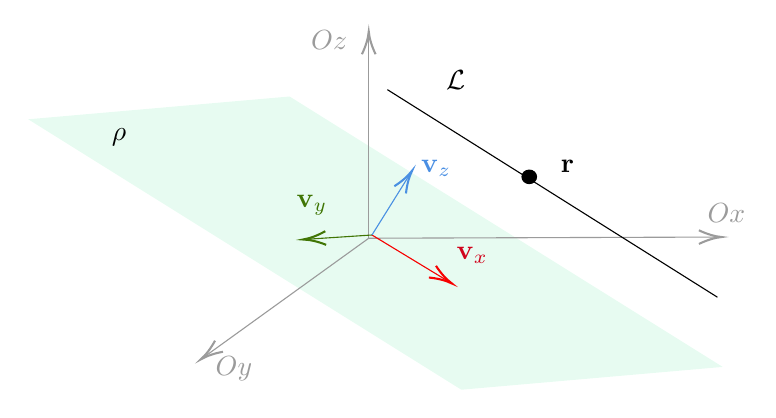
\begin{tikzpicture}[x=0.75pt,y=0.75pt,yscale=-1,xscale=1]
			%uncomment if require: \path (0,300); %set diagram left start at 0, and has height of 300
			
			%Shape: Parallelogram [id:dp12923406047287678] 
			\draw  [draw opacity=0][fill={rgb, 255:red, 82; green, 230; blue, 155 }  ,fill opacity=0.14 ] (232.86,50.29) -- (441.53,180.58) -- (315.61,191.56) -- (106.94,61.27) -- cycle ;
			%Straight Lines [id:da09775279086463651] 
			\draw [color={rgb, 255:red, 155; green, 155; blue, 155 }  ,draw opacity=1 ]   (271,118.58) -- (439,118.01) ;
			\draw [shift={(441,118)}, rotate = 179.8] [color={rgb, 255:red, 155; green, 155; blue, 155 }  ,draw opacity=1 ][line width=0.75]    (10.93,-3.29) .. controls (6.95,-1.4) and (3.31,-0.3) .. (0,0) .. controls (3.31,0.3) and (6.95,1.4) .. (10.93,3.29)   ;
			%Straight Lines [id:da03412940385078733] 
			\draw [color={rgb, 255:red, 155; green, 155; blue, 155 }  ,draw opacity=1 ]   (271,118.58) -- (271,21) ;
			\draw [shift={(271,19)}, rotate = 90] [color={rgb, 255:red, 155; green, 155; blue, 155 }  ,draw opacity=1 ][line width=0.75]    (10.93,-3.29) .. controls (6.95,-1.4) and (3.31,-0.3) .. (0,0) .. controls (3.31,0.3) and (6.95,1.4) .. (10.93,3.29)   ;
			%Straight Lines [id:da5931721359389577] 
			\draw [color={rgb, 255:red, 155; green, 155; blue, 155 }  ,draw opacity=1 ]   (271,118.58) -- (191.62,175.83) ;
			\draw [shift={(190,177)}, rotate = 324.2] [color={rgb, 255:red, 155; green, 155; blue, 155 }  ,draw opacity=1 ][line width=0.75]    (10.93,-3.29) .. controls (6.95,-1.4) and (3.31,-0.3) .. (0,0) .. controls (3.31,0.3) and (6.95,1.4) .. (10.93,3.29)   ;
			%Straight Lines [id:da6368016285772775] 
			\draw [color={rgb, 255:red, 65; green, 117; blue, 5 }  ,draw opacity=1 ]   (272.55,117.02) -- (241.36,119.06) ;
			\draw [shift={(239.36,119.19)}, rotate = 356.26] [color={rgb, 255:red, 65; green, 117; blue, 5 }  ,draw opacity=1 ][line width=0.75]    (10.93,-3.29) .. controls (6.95,-1.4) and (3.31,-0.3) .. (0,0) .. controls (3.31,0.3) and (6.95,1.4) .. (10.93,3.29)   ;
			%Straight Lines [id:da4069337085595317] 
			\draw [color={rgb, 255:red, 247; green, 0; blue, 0 }  ,draw opacity=1 ]   (272.55,117.02) -- (297.37,132.08) -- (309.32,139.32) ;
			\draw [shift={(311.03,140.36)}, rotate = 211.24] [color={rgb, 255:red, 247; green, 0; blue, 0 }  ,draw opacity=1 ][line width=0.75]    (10.93,-3.29) .. controls (6.95,-1.4) and (3.31,-0.3) .. (0,0) .. controls (3.31,0.3) and (6.95,1.4) .. (10.93,3.29)   ;
			%Straight Lines [id:da9797077411347257] 
			\draw [color={rgb, 255:red, 74; green, 144; blue, 226 }  ,draw opacity=1 ]   (272.55,117.02) -- (290.86,87.69) ;
			\draw [shift={(291.92,85.99)}, rotate = 121.98] [color={rgb, 255:red, 74; green, 144; blue, 226 }  ,draw opacity=1 ][line width=0.75]    (10.93,-3.29) .. controls (6.95,-1.4) and (3.31,-0.3) .. (0,0) .. controls (3.31,0.3) and (6.95,1.4) .. (10.93,3.29)   ;
			%Straight Lines [id:da7904650311794801] 
			\draw    (280,47) -- (439,147) ;
			%Shape: Ellipse [id:dp3940510086036726] 
			\draw  [fill={rgb, 255:red, 0; green, 0; blue, 0 }  ,fill opacity=1 ] (344.83,89) .. controls (344.83,87.21) and (346.4,85.75) .. (348.33,85.75) .. controls (350.27,85.75) and (351.83,87.21) .. (351.83,89) .. controls (351.83,90.79) and (350.27,92.25) .. (348.33,92.25) .. controls (346.4,92.25) and (344.83,90.79) .. (344.83,89) -- cycle ;
			
			
			% Text Node
			\draw (433,100.4) node [anchor=north west][inner sep=0.75pt]  [color={rgb, 255:red, 155; green, 155; blue, 155 }  ,opacity=1 ]  {$Ox$};
			% Text Node
			\draw (242,17.4) node [anchor=north west][inner sep=0.75pt]  [color={rgb, 255:red, 155; green, 155; blue, 155 }  ,opacity=1 ]  {$Oz$};
			% Text Node
			\draw (196,174.4) node [anchor=north west][inner sep=0.75pt]  [color={rgb, 255:red, 155; green, 155; blue, 155 }  ,opacity=1 ]  {$Oy$};
			% Text Node
			\draw (235,96.4) node [anchor=north west][inner sep=0.75pt]  [color={rgb, 255:red, 155; green, 155; blue, 155 }  ,opacity=1 ]  {$\textcolor[rgb]{0.25,0.46,0.02}{\mathbf v}\textcolor[rgb]{0.25,0.46,0.02}{_{y}}$};
			% Text Node
			\draw (312.03,121.61) node [anchor=north west][inner sep=0.75pt]  [color={rgb, 255:red, 155; green, 155; blue, 155 }  ,opacity=1 ]  {$\textcolor[rgb]{0.82,0.01,0.11}{\mathbf v}\textcolor[rgb]{0.82,0.01,0.11}{_{x}}$};
			% Text Node
			\draw (295.03,79.61) node [anchor=north west][inner sep=0.75pt]  [color={rgb, 255:red, 155; green, 155; blue, 155 }  ,opacity=1 ]  {$\textcolor[rgb]{0.29,0.56,0.89}{\mathbf v}\textcolor[rgb]{0.29,0.56,0.89}{_{z}}$};
			% Text Node
			\draw (307,36.4) node [anchor=north west][inner sep=0.75pt]    {$\mathcal L$};
			% Text Node
			\draw (146,64.4) node [anchor=north west][inner sep=0.75pt]    {$\rho $};
			
			% Text Node
			\draw (362.33,79.73) node [anchor=north west][inner sep=0.75pt]    {$\mathbf r$};
			
		\end{tikzpicture}
		
		$\mathcal{L}$ is defined by a point $\mathbf r \in \mathcal{L}$ and vector $\mathbf u \parallel \mathcal{L}$. Plane $\rho$ passes through the origin and is defined by its normal $\mathbf v_z$ and tangents $\mathbf v_x$, $\mathbf v_y$.
		
	\end{flushleft}
\end{frame}


\begin{frame}{Line parallel to a plane}
	% \framesubtitle{Part 1}
	\begin{flushleft}
		
		First, let us observe that for the line $\mathcal{L}$ to be parallel to the plane, it has to be orthogonal to the plane's normal, i.e. $\mathbf v_z$. Which is the same as $\mathbf u \cdot \mathbf v_z = 0$.
		
		\bigskip
		
		Second, let us find how $\mathbf r$ can be expressed as a linear combination of $\mathbf v_x$, $\mathbf v_y$ and $\mathbf v_z$:
		
		\begin{equation}
			\mathbf r = \alpha_x \mathbf v_x + \alpha_y \mathbf v_y + \alpha_z \mathbf v_z
		\end{equation}
		
		\begin{equation}
			\begin{bmatrix}
				\alpha_x \\ \alpha_y \\ \alpha_z
			\end{bmatrix}
			=
			\begin{bmatrix}
				\mathbf v_x &  \mathbf v_y &  \mathbf v_z
			\end{bmatrix}^{-1}
			\mathbf r
		\end{equation}
	
		Now consider point $\mathbf r_\rho = \alpha_x \mathbf v_x + \alpha_y \mathbf v_y \in \rho$. It is the closest point on $\rho$ to the point $\mathbf r$. So the distance to the line is $||\mathbf r_\rho - \mathbf r || = || \alpha_z \mathbf v_z || = \alpha_z || \mathbf v_z ||$ and if $|| \mathbf v_z || = 1$, then the distance between line and plane is $ \alpha_z$.
		
	\end{flushleft}
\end{frame}


\begin{frame}{Line parallel to a plane}
	% \framesubtitle{Part 1}
	\begin{flushleft}
		
		Wait, but why is $\mathbf r_\rho = \alpha_x \mathbf v_x + \alpha_y \mathbf v_y \in \rho$ the closest point to on $\rho$ to the point $\mathbf r$?
		
		\bigskip
		
		Assume the opposite. Let $\mathbf y = \mathbf r_\rho + \beta_x \mathbf v_x + \beta_y \mathbf v_y$ be the point which is closer to $\mathbf r$. Let us find distances $||\mathbf r_\rho - \mathbf r||$ and $||\mathbf y - \mathbf r||$:
		
		\begin{equation}
			||\mathbf r_\rho - \mathbf r|| = ||\alpha_z \mathbf v_z|| = \alpha_z
		\end{equation}
	
		\begin{equation}
		||\mathbf y - \mathbf r|| = ||\beta_x \mathbf v_x + \beta_y \mathbf v_y + \alpha_z \mathbf v_z|| \geq \alpha_z
		\end{equation}
	
	Note that the last inequality is due to Pythagorean theorem, as both $ \mathbf v_x$ and $ \mathbf v_y$ are orthogonal to $ \mathbf v_z$. \qed
		
	\end{flushleft}
\end{frame}



\begin{frame}{Line and plane intersection}
	% \framesubtitle{Part 1}
	\begin{flushleft}
		
		Consider a plane $\rho$ and a line $\mathcal L$ passing through the point $\mathbf r$. Find coordinates of  the point of intersection $\mathbf p$  of the plane and line.
		
		\tikzset{every picture/.style={line width=0.75pt}} %set default line width to 0.75pt        
		
		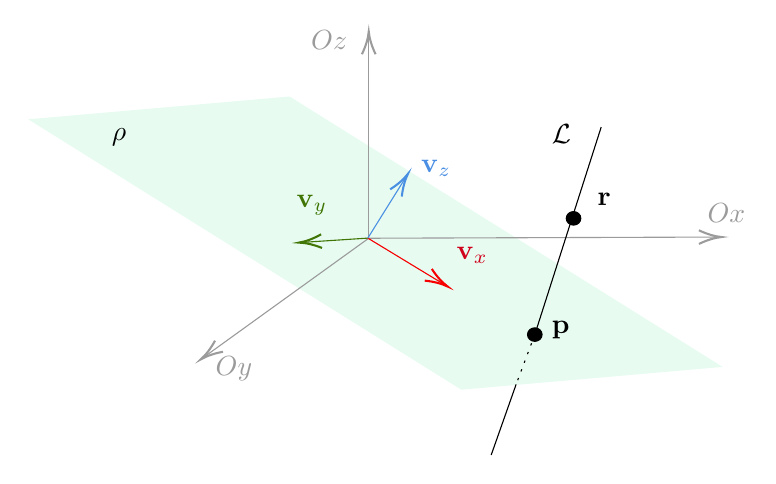
\begin{tikzpicture}[x=0.75pt,y=0.75pt,yscale=-1,xscale=1]
			%uncomment if require: \path (0,300); %set diagram left start at 0, and has height of 300
			
			%Shape: Parallelogram [id:dp8306904325015949] 
			\draw  [draw opacity=0][fill={rgb, 255:red, 82; green, 230; blue, 155 }  ,fill opacity=0.14 ] (232.86,50.29) -- (441.53,180.58) -- (315.61,191.56) -- (106.94,61.27) -- cycle ;
			%Straight Lines [id:da08630072901249775] 
			\draw [color={rgb, 255:red, 155; green, 155; blue, 155 }  ,draw opacity=1 ]   (271,118.58) -- (439,118.01) ;
			\draw [shift={(441,118)}, rotate = 179.8] [color={rgb, 255:red, 155; green, 155; blue, 155 }  ,draw opacity=1 ][line width=0.75]    (10.93,-3.29) .. controls (6.95,-1.4) and (3.31,-0.3) .. (0,0) .. controls (3.31,0.3) and (6.95,1.4) .. (10.93,3.29)   ;
			%Straight Lines [id:da9854878480389433] 
			\draw [color={rgb, 255:red, 155; green, 155; blue, 155 }  ,draw opacity=1 ]   (271,118.58) -- (271,21) ;
			\draw [shift={(271,19)}, rotate = 90] [color={rgb, 255:red, 155; green, 155; blue, 155 }  ,draw opacity=1 ][line width=0.75]    (10.93,-3.29) .. controls (6.95,-1.4) and (3.31,-0.3) .. (0,0) .. controls (3.31,0.3) and (6.95,1.4) .. (10.93,3.29)   ;
			%Straight Lines [id:da627752815801145] 
			\draw [color={rgb, 255:red, 155; green, 155; blue, 155 }  ,draw opacity=1 ]   (271,118.58) -- (191.62,175.83) ;
			\draw [shift={(190,177)}, rotate = 324.2] [color={rgb, 255:red, 155; green, 155; blue, 155 }  ,draw opacity=1 ][line width=0.75]    (10.93,-3.29) .. controls (6.95,-1.4) and (3.31,-0.3) .. (0,0) .. controls (3.31,0.3) and (6.95,1.4) .. (10.93,3.29)   ;
			%Straight Lines [id:da6295398558839993] 
			\draw    (383,65) -- (351,165) ;
			%Straight Lines [id:da41482544339087757] 
			\draw  [dash pattern={on 0.84pt off 2.51pt}]  (351,165) -- (342,189) ;
			%Straight Lines [id:da15822326568287548] 
			\draw    (342,189) -- (330,223) ;
			%Shape: Ellipse [id:dp7921309425219902] 
			\draw  [fill={rgb, 255:red, 0; green, 0; blue, 0 }  ,fill opacity=1 ] (347.5,165) .. controls (347.5,163.21) and (349.07,161.75) .. (351,161.75) .. controls (352.93,161.75) and (354.5,163.21) .. (354.5,165) .. controls (354.5,166.79) and (352.93,168.25) .. (351,168.25) .. controls (349.07,168.25) and (347.5,166.79) .. (347.5,165) -- cycle ;
			%Straight Lines [id:da24136093195468877] 
			\draw [color={rgb, 255:red, 65; green, 117; blue, 5 }  ,draw opacity=1 ]   (270.55,118.52) -- (239.36,120.56) ;
			\draw [shift={(237.36,120.69)}, rotate = 356.26] [color={rgb, 255:red, 65; green, 117; blue, 5 }  ,draw opacity=1 ][line width=0.75]    (10.93,-3.29) .. controls (6.95,-1.4) and (3.31,-0.3) .. (0,0) .. controls (3.31,0.3) and (6.95,1.4) .. (10.93,3.29)   ;
			%Straight Lines [id:da5492771226172424] 
			\draw [color={rgb, 255:red, 247; green, 0; blue, 0 }  ,draw opacity=1 ]   (270.55,118.52) -- (295.37,133.58) -- (307.32,140.82) ;
			\draw [shift={(309.03,141.86)}, rotate = 211.24] [color={rgb, 255:red, 247; green, 0; blue, 0 }  ,draw opacity=1 ][line width=0.75]    (10.93,-3.29) .. controls (6.95,-1.4) and (3.31,-0.3) .. (0,0) .. controls (3.31,0.3) and (6.95,1.4) .. (10.93,3.29)   ;
			%Straight Lines [id:da24062437415238236] 
			\draw [color={rgb, 255:red, 74; green, 144; blue, 226 }  ,draw opacity=1 ]   (270.55,118.52) -- (288.86,89.19) ;
			\draw [shift={(289.92,87.49)}, rotate = 121.98] [color={rgb, 255:red, 74; green, 144; blue, 226 }  ,draw opacity=1 ][line width=0.75]    (10.93,-3.29) .. controls (6.95,-1.4) and (3.31,-0.3) .. (0,0) .. controls (3.31,0.3) and (6.95,1.4) .. (10.93,3.29)   ;
			%Shape: Ellipse [id:dp929005244530769] 
			\draw  [fill={rgb, 255:red, 0; green, 0; blue, 0 }  ,fill opacity=1 ] (366.17,109) .. controls (366.17,107.21) and (367.73,105.75) .. (369.67,105.75) .. controls (371.6,105.75) and (373.17,107.21) .. (373.17,109) .. controls (373.17,110.79) and (371.6,112.25) .. (369.67,112.25) .. controls (367.73,112.25) and (366.17,110.79) .. (366.17,109) -- cycle ;
			
			% Text Node
			\draw (433,100.4) node [anchor=north west][inner sep=0.75pt]  [color={rgb, 255:red, 155; green, 155; blue, 155 }  ,opacity=1 ]  {$Ox$};
			% Text Node
			\draw (242,17.4) node [anchor=north west][inner sep=0.75pt]  [color={rgb, 255:red, 155; green, 155; blue, 155 }  ,opacity=1 ]  {$Oz$};
			% Text Node
			\draw (196,174.4) node [anchor=north west][inner sep=0.75pt]  [color={rgb, 255:red, 155; green, 155; blue, 155 }  ,opacity=1 ]  {$Oy$};
			% Text Node
			\draw (235,96.4) node [anchor=north west][inner sep=0.75pt]  [color={rgb, 255:red, 155; green, 155; blue, 155 }  ,opacity=1 ]  {$\textcolor[rgb]{0.25,0.46,0.02}{\mathbf v}\textcolor[rgb]{0.25,0.46,0.02}{_{y}}$};
			% Text Node
			\draw (312.03,121.61) node [anchor=north west][inner sep=0.75pt]  [color={rgb, 255:red, 155; green, 155; blue, 155 }  ,opacity=1 ]  {$\textcolor[rgb]{0.82,0.01,0.11}{\mathbf v}\textcolor[rgb]{0.82,0.01,0.11}{_{x}}$};
			% Text Node
			\draw (295.03,79.61) node [anchor=north west][inner sep=0.75pt]  [color={rgb, 255:red, 155; green, 155; blue, 155 }  ,opacity=1 ]  {$\textcolor[rgb]{0.29,0.56,0.89}{\mathbf v}\textcolor[rgb]{0.29,0.56,0.89}{_{z}}$};
			% Text Node
			\draw (358,62.4) node [anchor=north west][inner sep=0.75pt]    {$\mathcal L$};
			% Text Node
			\draw (146,64.4) node [anchor=north west][inner sep=0.75pt]    {$\rho $};
			% Text Node
			\draw (358,157.4) node [anchor=north west][inner sep=0.75pt]    {$\mathbf p$};
			% Text Node
			\draw (380,95.4) node [anchor=north west][inner sep=0.75pt]    {$\mathbf r$};
			
			
		\end{tikzpicture}
		
		Direction of the $\mathcal L$ is defined by vector $\mathbf u$. Orientation of $\rho$ is given by vector $\mathbf v_z$.
		
	\end{flushleft}
\end{frame}


\begin{frame}{Line and plane intersection}
	% \framesubtitle{Part 1}
	\begin{flushleft}
		
		We know that $\mathbf p \in \mathcal L$, so $\mathbf p = \textcolor{mygreen}{\lambda} \mathbf u + \mathbf r$.
		
		\bigskip
		
		And $\mathbf p \in \rho$, so $\mathbf p \cdot \mathbf v_z = 0$, hence:
		%
		\begin{align}
			(\lambda \mathbf u + \mathbf r) \cdot \mathbf v_z = 0 \\
			\lambda \mathbf u \cdot \mathbf v_z + \mathbf r \cdot \mathbf v_z = 0 \\
			\textcolor{mygreen}{\lambda} = - \frac{\mathbf r \cdot \mathbf v_z}{ \mathbf u \cdot \mathbf v_z}
		\end{align}
		
		\bigskip
		
		And thus we get our solution:
		
		\begin{equation}
			\mathbf p =\textcolor{mygreen}{
			 - \frac{\mathbf r \cdot \mathbf v_z}{ \mathbf u \cdot \mathbf v_z}
		     } \mathbf u + \mathbf r
		\end{equation}
		
	\end{flushleft}
\end{frame}


\begin{frame}{Two plane intersection}
	% \framesubtitle{Part 1}
	\begin{flushleft}
		
		Consider two planes $\rho_1$ and $\rho_2$, find a line $\mathcal L$ that lies on their intersection. The plane $\rho_1$ is given by its normal $\mathbf  n_1$ and plane $\rho_2$ is given by its normal $\mathbf  n_2$. Direction of $\mathcal L$ is given by a vector $\mathbf u$.	
		
		\tikzset{every picture/.style={line width=0.75pt}} %set default line width to 0.75pt        
		
		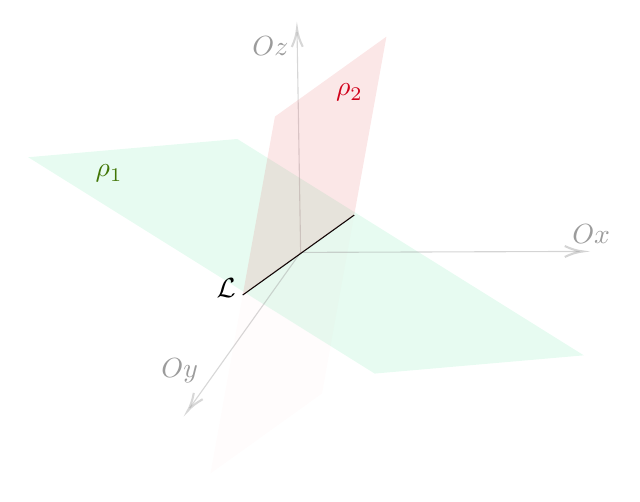
\begin{tikzpicture}[x=0.75pt,y=0.75pt,yscale=-0.8,xscale=0.8]
			%uncomment if require: \path (0,302); %set diagram left start at 0, and has height of 302
			
			%Shape: Parallelogram [id:dp5144316665751045] 
			\draw  [draw opacity=0][fill={rgb, 255:red, 82; green, 230; blue, 155 }  ,fill opacity=0.14 ] (227.86,84.29) -- (436.53,214.58) -- (310.61,225.56) -- (101.94,95.27) -- cycle ;
			%Straight Lines [id:da4983969525113505] 
			\draw [color={rgb, 255:red, 155; green, 155; blue, 155 }  ,draw opacity=0.43 ]   (266,152.58) -- (434,152.01) ;
			\draw [shift={(436,152)}, rotate = 179.8] [color={rgb, 255:red, 155; green, 155; blue, 155 }  ,draw opacity=0.43 ][line width=0.75]    (10.93,-3.29) .. controls (6.95,-1.4) and (3.31,-0.3) .. (0,0) .. controls (3.31,0.3) and (6.95,1.4) .. (10.93,3.29)   ;
			%Straight Lines [id:da7492357808708827] 
			\draw [color={rgb, 255:red, 155; green, 155; blue, 155 }  ,draw opacity=0.4 ]   (266,152.58) -- (263.89,23.47) -- (263.83,19.87) ;
			\draw [shift={(263.8,17.87)}, rotate = 89.06] [color={rgb, 255:red, 155; green, 155; blue, 155 }  ,draw opacity=0.4 ][line width=0.75]    (10.93,-3.29) .. controls (6.95,-1.4) and (3.31,-0.3) .. (0,0) .. controls (3.31,0.3) and (6.95,1.4) .. (10.93,3.29)   ;
			%Straight Lines [id:da7027273717077036] 
			\draw [color={rgb, 255:red, 155; green, 155; blue, 155 }  ,draw opacity=0.4 ]   (266,152.58) -- (208.47,233.31) -- (206.58,235.97) -- (203.61,240.13) -- (199.16,246.37) ;
			\draw [shift={(198,248)}, rotate = 305.48] [color={rgb, 255:red, 155; green, 155; blue, 155 }  ,draw opacity=0.4 ][line width=0.75]    (10.93,-3.29) .. controls (6.95,-1.4) and (3.31,-0.3) .. (0,0) .. controls (3.31,0.3) and (6.95,1.4) .. (10.93,3.29)   ;
			%Straight Lines [id:da7766543379890278] 
			\draw    (298.26,130.09) -- (231.11,178.25) ;
			%Shape: Parallelogram [id:dp7892017648177252] 
			\draw  [draw opacity=0][fill={rgb, 255:red, 230; green, 82; blue, 87 }  ,fill opacity=0.14 ] (250.51,70.81) -- (317.66,22.65) -- (298.26,130.09) -- (231.11,178.25) -- cycle ;
			%Shape: Parallelogram [id:dp8095142391921688] 
			\draw  [draw opacity=0][fill={rgb, 255:red, 230; green, 82; blue, 87 }  ,fill opacity=0.02 ] (231.11,178.25) -- (298.26,130.09) -- (278.85,237.54) -- (211.71,285.7) -- cycle ;
			
			% Text Node
			\draw (428,134.4) node [anchor=north west][inner sep=0.75pt]  [color={rgb, 255:red, 155; green, 155; blue, 155 }  ,opacity=1 ]  {$Ox$};
			% Text Node
			\draw (235.4,21) node [anchor=north west][inner sep=0.75pt]  [color={rgb, 255:red, 155; green, 155; blue, 155 }  ,opacity=1 ]  {$Oz$};
			% Text Node
			\draw (180.6,214.8) node [anchor=north west][inner sep=0.75pt]  [color={rgb, 255:red, 155; green, 155; blue, 155 }  ,opacity=1 ]  {$Oy$};
			% Text Node
			\draw (213.8,166.8) node [anchor=north west][inner sep=0.75pt]    {$\mathcal L$};
			% Text Node
			\draw (141,98.4) node [anchor=north west][inner sep=0.75pt]  [color={rgb, 255:red, 65; green, 117; blue, 5 }  ,opacity=1 ]  {$\rho _{1}$};
			% Text Node
			\draw (285.8,49.6) node [anchor=north west][inner sep=0.75pt]  [color={rgb, 255:red, 208; green, 2; blue, 27 }  ,opacity=1 ]  {$\rho _{2}$};
			
			
		\end{tikzpicture}
			
	\end{flushleft}
\end{frame}


\begin{frame}{Two plane intersection}
	% \framesubtitle{Part 1}
	\begin{flushleft}
		
		Since $0 \in \rho_1$ and $0 \in \rho_2$, meaning that $0 \in \mathcal L$.
		
		Note that $\mathbf u \in \rho_1$ and $\mathbf u \in \rho_2$. Hence:
		
		\begin{equation}
			\mathbf u \cdot \mathbf n_1 = 0; \ \ \ \mathbf u \cdot \mathbf n_2 = 0
		\end{equation} 
		
		And we know how to find a vector in $\mathbb R^3$ perpendicular to two other non-parallel vectors in $\mathbb R^3$: we use cross-product.
		
		\begin{equation}
			\mathbf u = \mathbf n_1 \times \mathbf n_2
		\end{equation} 		
		
		If we need $\mathbf u$ to be unit length, we normalize it. 
		
	\end{flushleft}
\end{frame}



%\begin{frame}{Read more}
%
%\begin{itemize}
%\item \bref{https://mathinsight.org/matrices_determinants_multivariable_calculus}{mathinsight.org/matrices\_determinants}
%
%\item \bref{https://en.wikipedia.org/wiki/Determinant}{en.wikipedia.org/wiki/Determinant}
%
%\end{itemize}
%
%\end{frame}



\begin{frame}{Thank you!}
\centerline{Lecture slides are available via Moodle.}
\bigskip
\centerline{You can help improve these slides at:}
\centerline{\mygit}
\bigskip
\centerline{Check Moodle for additional links, videos, textbook suggestions.}
\bigskip

\centerline{\textcolor{black}{\qrcode[height=1.6in]{https://github.com/SergeiSa/Extra-math-for-high-school}}}

\end{frame}

\end{document}
